\chapter{Principy a historie regulárních výrazů}\label{sec:Principle}

Tato kapitola se zabývá definicí regulárních výrazů, jak fungují a jak se jednotlivé implementace mohu lišit. 
Součástí jejích implementace, provází několik pojmů z teoretické informatiky, odkud pocházejí.
Hlavně se jedná o \textbf{Konečné automaty} a \textbf{Thompsonovo sestrojení}.
%Následovně si vysvětlíme, jak lze zjednodušit pochopení těchto výrazů, popřípadě jak rychle najít chybu ve vlastním výrazu. 

%Předtím než si vysvětlíme blíže jak fungují samotné regulární výrazy, je potřeba si objasnit význam několika pojmů z teoretické informatiky.



\section{Formální jazyk}
Formální jazyk je libovolná množina konečných slov nad určitou abecedou. 
Slova chápeme jako řetězce znaků, která jsou přijímaná zadaným jazykem.
Tato slova musí být sice konečná ale množina těchto slov může být nekonečná. 
Tyto jazyky mohou být definovány regulárními výrazy, formální gramatikou,
konečnými automaty a dalšími. Regulární jazyky jsou pak jednou z možných definic formálních jazyků.

\section{Konečný automat}\label{sec:FiniteAutomaton}
Ve spojení s regulárními výrazy se často pojí konečné automaty, jedná se o další oblast v teoretické informatice.
Tato práce implementuje regulární výrazy právě ve forme konečných automatů.

Zjednodušeně se dá říct, že konečný automat je model jednoduchého počítače, který má určitý počet stavů a přechodů \cite{Havrlant}. 

Stavy jsou typicky zakreslovány jako kružnice, a každý automat musí obsahovat alespoň jeden počáteční stav, ale může jich také obsahovat více. 
To samé platí pro konečný/é stav/y. 
Konečné stavy se také vyznačují jako kruh, ale z dvojitou čárou. 
Počáteční stavy, jsou označovány jako stav, do kterého vede šipka, která ale nevychází z jiného stavu.
Přechody jsou pak šipky vedoucí z jednoho stavu do druhého, jsou označeny přechodovým symbolem.
Avšak přechod může odkazovat na stejný stav, ze kterého vychází.
Tyto přechody nám říkají že pokud chceme přejít z jednoho stavu do druhého, tak musíme v přijímaném slově se posunout o daný symbol. 
Pokud to není možné, tak nemůžeme přejít do tohoto stavu.

Tyto automaty se dělí na \textbf{deterministické} a \textbf{nedeterministické}, zkráceně \textbf{DKA} (deterministický konečný automat) a \textbf{NKA} (nedeterministický konečný automat).
DKA mohou mít v daném stavu pro každý znak abecedy \textbf{maximálně} jeden přechod, dále \textbf{nemohou obsahovat tzv. prázdný znak} často označovaný řeckým písmenem epsilon $\epsilon$.
Příklad tohoto automatu je možno vidět na obrázku \ref{fig:DFAex}.
NKA naopak obojí umožňují. 
Prázdné znaky slouží pro změnu stavu bez změny aktuální pozice v hledaném slově. 
Pro ukázku si můžeme porovnat dva ekvivalentní konečné automaty,
NKA na obrázku \ref{fig:NFAex} a DKA na obrázku \ref{fig:DFAex}.
Nakonec je dobré podotknout, že každý NKA lze převést na ekvivalentní DKA.

\begin{figure}[!h]
	\centering
	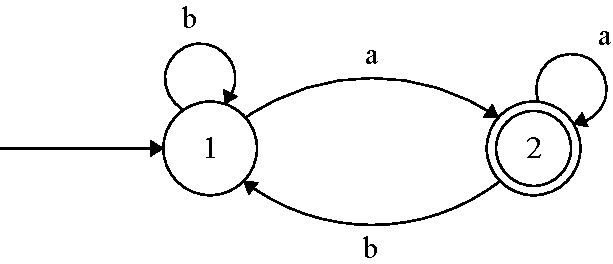
\includegraphics[width=0.6\textwidth]{Figures/DFA_example.pdf}
	\caption{Příklad deterministického automatu přijímající slova obsahující písmena z abecedy \{a, b\} končící písmenem a}
	\label{fig:DFAex}
\end{figure}

\begin{figure}[!h]
	\centering
	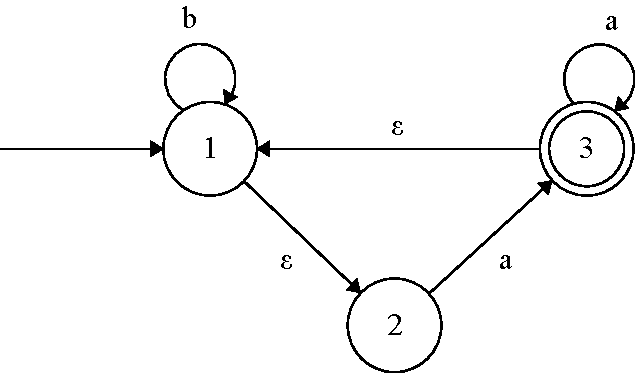
\includegraphics[width=0.6\textwidth]{Figures/NFA_example.pdf}
	\caption{Příklad nedeterministického automatu ekvivalentního k předchozímu deterministickému}
	\label{fig:NFAex}
\end{figure}

\section{Bezkontextová gramatika}
Součástí této práce je i využití Bezkontextové gramatiky a jelikož spadají pod teoretickou informatiku, 
tak si zkráceně vysvětlíme tuto oblast.

Bezkontextová gramatika, je další z možných definic formálních jazyků. Je určená konečnou množinou \textbf{neterminálních symbolů} (proměnných), konečnou množinou \textbf{terminálních symbolů}, která nesmí mít žádné prvky společné s předchozí množinou.
Dále \textbf{počátečním neterminálem} s konečnou množinou \textbf{přepisových pravidel}\cite{MUNIFL}.

$A \longrightarrow \beta$

\noindent 
kde A je neterminál a $\beta$ je řetězec složený z terminálů a/nebo neterminálů. 
Dále šipka indikuje \textbf{přepsání} tj. levá strana se přepisuje na stranu pravou.
Konečný generovaný řetězec danou gramatikou, je pouze tvořen terminálními symboly.
Aby mohl být řetězec přijímaný zadanou gramatikou, musí ho být schopná tato gramatika vygenerovat.

\section{Vznik, implementace a vzory}
Regulární výrazy byly poprvé nadefinovány Americkým matematikem \textbf{Stephan Cole Kleene}, jako regulární jazyky. 
Dále se aplikovali v teoretické informatice, jako podkategorie \textbf{teorie automatů} a součást \textbf{formálních jazyků}.
Ačkoliv byly nadefinovány začátkem padesátých let, tak jejich využití v počítačích nastalo až na konci šedesátých let a to v 
jedním z nejznámějších operačních systémů UNIX.

\subsection*{Thompsonovo sestrojení}

První kdo navrhl implementaci používanou v počítačích byl \textbf{Ken Thompson}.
Principem byl převod regulárního výrazu na NKA.
Tato metoda se často používá v podobné či stejné formě doposud.
Algoritmus se pojmenoval \textbf{Thompson's construction} (Thompsonovo sestrojení), který převádí textovou reprezentaci výrazu na ekvivalentní nedeterministický automat.
Toto sestrojení je využito v této práci a blíže jej popisuje následující část textu.

NKA se běžně využívá, jelikož je poměrně jednoduchý na implementaci a
také oproti DKA využívá \textbf{zpětného krokování (backtracking)} a povoluje složitější operace jako je \textbf{rozhlédnutí se kolem sebe (lookaround)}.
Zpětné krokování je důležité pro NKA, jelikož neexistuje jednoznačná cesta vyhodnocení.
DKA mají výhodu že jsou rychlejší, ale jsou typicky větší než jejich ekvivalentní NKA a neumožňují některé složitější operace.
Také nepotřebují zpětné krokování, jelikož jejich cesta je deterministická tzn. existuje vždy jen jedna cesta pro hledané slovo.
Někdy se ale využívá kombinace DKA i NKA, kdy DKA se využije kvůli vyšší rychlosti vyhledání daného slova a pokud bylo slovo nalezeno, 
tak se použije NKA pro jejich rozšířené možnosti.

Výsledný NKA po Thompsonově sestrojení má právě jeden vstupní a výstupní stav. 
Thompsonovo sestrojení dále definuje následující pravidla.

Prázdný výraz \textit{$\epsilon$}, je převedený na vstupní stav, přechod \textit{$\epsilon$} a konečný stav.
Výsledný konečný automat je na obrázku \ref{fig:NFAepsilon}.
\begin{figure}[!h]
	\centering
	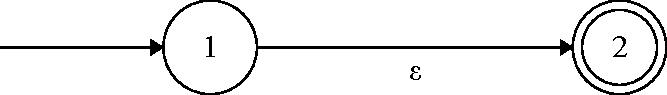
\includegraphics[width=0.5\textwidth]{Figures/NFA_epsilon.pdf}
	\caption{Převedený prázdný výraz \textbf{$\epsilon$}}
	\label{fig:NFAepsilon}
\end{figure}

Výraz \textit{a}, je převedený podobně jako prázdný výraz, ale s rozdílem přechodu \textit{a} místo \textit{$\epsilon$}.
Konečný automat, který nám vznikne je ukázán na obrázku \ref{fig:NFAa}.
\begin{figure}[!h]
	\centering
	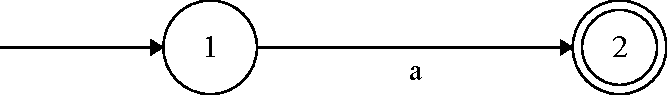
\includegraphics[width=0.5\textwidth]{Figures/NFA_a.pdf}
	\caption{Převedený výraz \textbf{a}}
	\label{fig:NFAa}
\end{figure}

Pro zadaný výraz \textbf{s|t}, kdy \textit{s} je levá strana varianty a \textit{t} je pravá strana varianty, platí že ze stavu \textit{q} (počáteční stav) vedou dva přechody
\textit{$\epsilon$} na počáteční stavy variant \textit{s} a \textit{t}. Z těchto počátečních stavů dále pokračuje sekvence stavů \textit{N(s)} pro \textit{s} a \textit{N(t)} pro \textit{t}.
Konce variant \textit{s} a \textit{t} mají jediný přechod \textit{$\epsilon$} na konečný stav \textit{f}.
Na obrázku \ref{fig:NFAunion} je vyobrazen výsledný NKA, 
kde skupina stavů v zelené části je \textit{s} a červená skupina je \textit{t}.
\begin{figure}[!h]
	\centering
	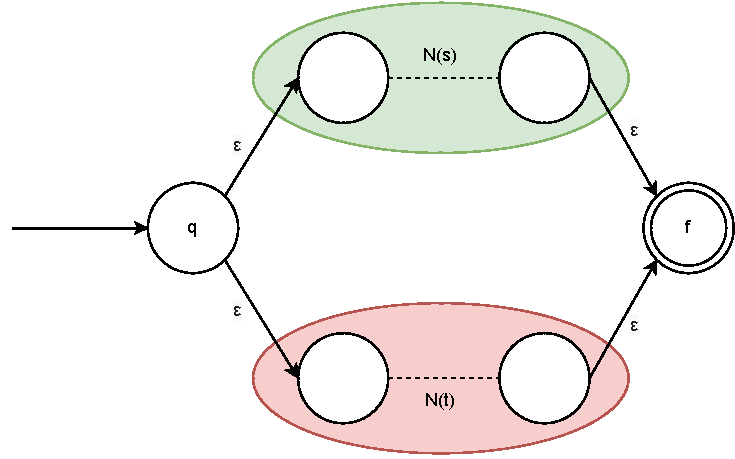
\includegraphics[width=0.6\textwidth]{Figures/NFA_union.pdf}
	\caption{Převedený výraz \textbf{s|t}}
	\label{fig:NFAunion}
\end{figure}

Další pravidla pro sestrojení lze například najít na anglické wikipedia stránce pro Thompsonovo sestrojení \cite{Wikipedia_2023}.

\subsection*{Základní vzory}
V Předchozích sekcích, již byly popsány základní konstrukce týkající se regulárních výrazů.
Tato sekce se zabývá jejich základními vzory.

Za nejjednodušší výraz lze považovat prázdný výraz, také označovaný jako $\epsilon$. 
Výrazy mohou obsahovat \textbf{téměř} libovolný znak, který bude přijímat slova s daným znakem. 
Avšak nemohou být použity znaky, které jsou rezervované, nebo-li jsou součástí syntaxe regulárních výrazů.
Chceme-li použít tyto znaky je potřeba použít znak \textbf{\\}. 
Takový znak se pak nazývá anglicky \textbf{escaped character}.

Iterace, je možnost jak lze opakovaně provádět nějakou operaci.
Například lze iterovat znak, skupinu a další konstrukce.
Prvním typem iterace je \textbf{*}, známa jako \textbf{Kleene star}, nebo-li kleene hvězda.
Tento druh iterace může mít počet opakování od \textbf{0} až do \textbf{n} iterací, taktéž se nezívá \textbf{nula nebo více}. 
Existují další 2 typy iterací a to je iterace typu \textbf{jedna nebo více} označována znakem + a \textbf{iterace v rozmezí}, která se značí \{od,do\}.

Operace \textbf{nebo} je dalším základním vzorem pro regulární výrazy. 
Jedná se o výběr mezi pravou a levou stranou. Oddělovacím znakem je typicky | podobně jako bitová operace \textbf{OR} v mnoha programovacích jazycích.

Dalšími základními konstrukty jsou například skupiny, které jsou obaleny v jednoduchých závorkách. 

\subsection*{Implementace v programovacích jazycích}\label{sec:impipl}

Dnes v podstatě každý programovací jazyk má v nějaké formě implementované zpracování regulárních výrazů.
Tato implementace se však často liší, sice základ bývá stejný, ale rozšířená syntaxe je často odlišná.
Může se tak stát to, že to co je podporované jedním jazykem, není podporované druhým.
Taktéž oproti původním regulárním výrazům, dnešní implementace obsahují mnohdy složitější
koncepce jako je rozhlédnutí se (Anglicky lookaround), nebo například rekurze.
Někdy sice jazyky sdílí jednu stejnou funkcionalitu, ale mohou se lišit syntaxí.

Rozhlédnutí se je již celkem pokročilá funkcionalita. 
Jejím principem je takzvaně, nezachytávání znaků při zpracovávání.
Typicky je dělíme podle směru a to na \textbf{dopředné} a \textbf{zpětné} rozhlédnutí.
Pak je dělíme podle podmínění a to na \textbf{kladné} a \textbf{negativní} rozhlédnutí.
Pokud máme kladné podmínění \textbf{musí} uzavřený výraz být splněný a pokud máme záporné tak \textbf{nesmí} být splněný.
V původní formě regulárních výrazů, tato funkce neexistovala.

Mnohdy je potřeba, nalezený řetězec rozdělit do skupin. 
Tuto možnost dnešní implementace také umožňují.
Chceme-li zdůraznit že zadaný podvýraz je skupinou, obalíme ho do závorek.
Tato vlastnost je žádaná, jelikož pak nemusíme hledat v již nalezeném řetězci další podřetězce.
Dají se dělit na zachytávající (capturing), pojmenované (named) a nezachytávající (non-capturing).
Pojmenované patří pod zachytávající, akorát jsou identifikovány pomocí názvu oproti indexu.
Poslední druh slouží čistě jako skupina pro regulární výraz, ale ve výsledku se neobjevuje.

\endinput